\scanpage{154}
\mspage{103}

encore sur une seule fibre ($f$ étant parfait, donc une $\unsure{W|\mathcal W}_{\unsure{\infty|0}}$-fibration, et $Y$ 0-connexe), soit

\[
 X_{y_0}\simeq\Omega(Y,y_0).
\]

Sa 0-connexité revient à l'hypothèse de 1-connexité de $Y$ (on n'a utilisé \inserted{\unsure{encore|même}} que celle de 0-connexité). Donc pour un contre-exemple, il suffit de prendre $Y$ 1-connexe et non $\infty$-connexe.

Le cas le plus simple est celui où $Y$ a le type d'homotopie de la sphère $S^2$, réalisé p. ex. par la catégorie ordonnée ci-contre à 6 sommets.

% slanted
\margin{C'est en somme cet exemple (à homotopie \unsure{top.} près) que je \unsure{révèle ici|vise ici|visais} \unsure{quand j'avais} \unsure{songé d'abord|d'abord} ; \unsure{voir} dans l'Appendice, p. \unsure{10-12|11-12}, un mot sur des catégories \uuline{finies}.}

\diagram{\begin{tikzcd}[ampersand replacement=\&,column sep=small,row sep=small]
 e_2^+\ {\bullet} \& {\bullet}\ e_2^-\\
 e_1^+\ {\bullet}\arrow[ur] \& {\bullet}\ e_1^-\arrow[ul,dashed]\\
 e_0^+\ {\bullet}\arrow[ur] \& {\bullet}\ e_0^-\arrow[ul,dashed]
\end{tikzcd}}

\figure{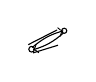
\begin{tikzpicture}[scale=.36]
\draw (0,0) circle (.10) (1.15,.65) circle (.09);
\draw[->] (.02,.06) to[bend left=12] (1.12,.65);
\draw[->] (1.12,.57) to[bend left=12] (.05,-.02);
\draw (-.12,.16)--(.90,.68) (.05,-.13)--(.93,.14);
\end{tikzpicture}}

Je résume le résultat obtenu

\uline{Proposition 10} Soit $Y$ une \inserted{petite} catégorie 1-connexe\inserted{, $y_0\in\mathrm{ob}\,Y$.} Alors $\underline{\mathrm{Ch}}(Y;y_0,-)$ est $W_\infty$-asphérique, mais n'est \inserted{pas} totalement $W_\infty$-asphérique si $Y$ elle-même n'est $\infty$-connexe \unsure{i.e.|ou} $W_\infty$-asphérique.

% slanted
\margin{Mais un exemple plus succinct est \diagram{\begin{tikzcd}[ampersand replacement=\&,column sep=small,row sep=small]
\&\&b\\
\unsure{\Psi|\Phi}={} \& a\arrow[ur]\arrow[dr]\&\\
\&\&c
\end{tikzcd}}, qui est $W_\infty$-asphérique, mais \uline{pas} totalement !}

On peut se demander si $Y$ $W_\infty$-asphérique implique que $\underline{\mathrm{Ch}}(Y;y_0,-)$ est tot. $W_\infty$-asphérique. J'en doute fort !
% archive sheet number: 154
